% Created 2016-05-03 tis 13:36
% Intended LaTeX compiler: pdflatex
\documentclass{scrartcl}
\usepackage[utf8]{inputenc}
\usepackage[T1]{fontenc}
\usepackage{graphicx}
\usepackage{grffile}
\usepackage{longtable}
\usepackage{wrapfig}
\usepackage{rotating}
\usepackage[normalem]{ulem}
\usepackage{amsmath}
\usepackage{textcomp}
\usepackage{amssymb}
\usepackage{capt-of}
\usepackage{hyperref}
\usepackage{khpreamble}
\author{Kjartan Halvorsen}
\date{Due Friday 2016-04-22}
\title{Computerized control - homework 4}
\hypersetup{
 pdfauthor={Kjartan Halvorsen},
 pdftitle={Computerized control - homework 4},
 pdfkeywords={},
 pdfsubject={},
 pdfcreator={Emacs 24.5.1 (Org mode 8.3.4)}, 
 pdflang={English}}
\begin{document}

\maketitle

\section*{Active suspension}
\label{sec:orgheadline5}
A so-called \emph{quarter model} for the suspension of a car is shown in figure \ref{fig:quarter}. The system consists of two masses, one is the mass of 1/4 of the car, the other is the much smaller suspension mass. The two masses are connected by two passive elements: a spring and a damper, as well as an active element: a linear force actuator. The suspension mass is connected with the ground via a spring, representing the tyre (sometimes there is also a damper included in the model of the tyre).
\begin{figure}
\begin{center}
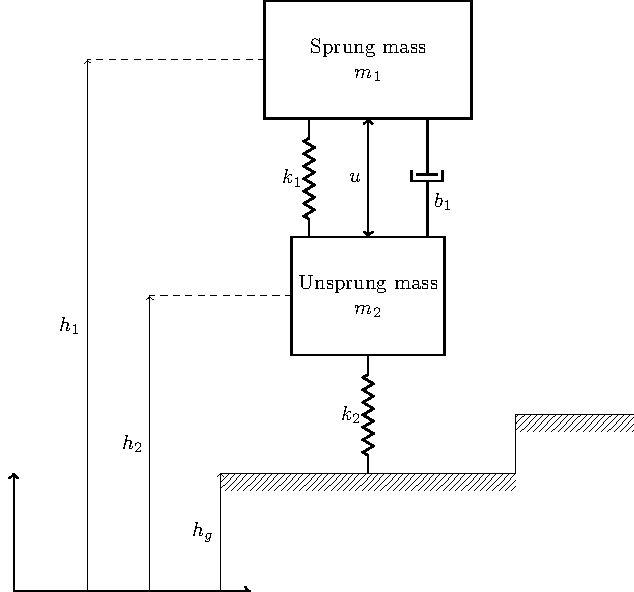
\includegraphics[width=0.35\linewidth]{../notes/figures/active-suspension-nodamper}
\caption{Active suspension model. The distances $z_1$, $z_2$ and $w$ are displacements from a static equilibrium. The displacements are measured with respect to a stationary frame of reference.}
\label{fig:quarter}
\end{center}
\end{figure}

A slightly more complex model is discussed \href{http://ctms.engin.umich.edu/CTMS/index.php?example=Suspension&section=ControlStateSpace}{here}. That model also includes a damping in the tyre. You are welcome to study the example. The parameter values are the same as for this homework assignment.

\subsection*{Determine the state space model}
\label{sec:orgheadline1}

\begin{enumerate}
\item Draw free-body diagrams for each of the two bodies, and set up the equation of motion of each of the two masses. Note that the variables \(z_1\), \(z_2\) and \(w\) are displacements from a static equilibrium, measured with respect to a stationary frame of reference. This means that the force acting on mass \(m_1\) from the spring between the two masses is \(F_s = m_1g -k_1(z_1-z_2)\), and the force acting on the suspension mass from the spring (tyre) between the suspension mass and ground is \(F_t= (m_1+m_2)g - k_2(z_2 - w)\). Moreover, the force in the damper is proportional with the relative velocity between the car and the suspension mass: \(F_d = -b_1(\dot{z}_1 - \dot{z}_2)\).
\item Show that the following state-space model of the system is obtained with the choice 
\[ x = \bbm x_1\\x_2\\x_3\\x_4 \ebm = \bbm z_1 - z_2\\ \dot{z}_1 - \dot{z}_2 \\ z_2\\ \dot{z}_2 \ebm \]
\begin{align*}
\dot{x} &= \bbm 0 & 1 & 0 & 0\\ 
-\Big(\frac{1}{m_1} + \frac{1}{m_2}\Big)k_1 & -\Big(\frac{1}{m_1} + \frac{1}{m_2}\Big)b_1 & \frac{k_2}{m_2} & 0\\
0 & 0 & 0 & 1\\
              \frac{k_1}{m_2} & \frac{b_1}{m_2} & - \frac{k_2}{m_2} & 0\ebm
              \bbm x_1\\x_2\\x_3\\x_4 \ebm + \bbm 0\\-\frac{k_2}{m_2}\\0\\\frac{k_2}{m_2} \ebm w + \bbm 0\\\frac{1}{m_1} + \frac{1}{m_2}\\0\\-\frac{1}{m_2} \ebm u \\
y &= \bbm 1 & 0 & 0 & 0 \ebm x.
\end{align*}
Note that the model has two inputs: The force from the active suspension \(u\), and the disturbance from the road \(w\).
\end{enumerate}
\subsection*{Simulate step-responses}
\label{sec:orgheadline2}
Implement the model in matlab. Use the following values for the parameters
\begin{center}
\begin{tabular}{l}
\(m1 = 2500\)\\
\(m2 = 320\)\\
\(k1 = 80000\)\\
\(k2 = 500000\)\\
\(b1 = 350\)\\
\end{tabular}
\end{center}
Note that the model has two input signals: The disturbance from the road, \(w\), and the actuator input \(u\). Simulate a step-response from each of the two input signals. Below is some code to help you
\begin{verbatim}
m1 = 2500;
m2 = 320;
k1 = 80000;
k2 = 500000;
b1 = 350;

A =   % Your code here
Bu = [0  
     1/m1+1/m2  
     0
     -1/m2 ];
Bw = [ 0
      -k2/m2
      0
      k2/m2];
C=[1 0 0 0];
D=[0];
sys_uy=ss(A,Bu,C,D);
sys_wy=ss(A,Bw,C,D);

% Step responses
figure(1)
clf
step(sys_uy, sys_wy)

% Simulate step response for first half second only
T = linspace(0, 0.5, 800);
figure(2)
clf
subplot(121)
stepplot(sys_uy, T);
title('Response from u')
xlabel('Time (seconds)')
ylabel('y (meters)')
subplot(122)
stepplot(sys_wy, T);
title('Response from w')
xlabel('Time (seconds)')
ylabel('y (meters)')
\end{verbatim}



\subsection*{Sample the system}
\label{sec:orgheadline3}
\begin{enumerate}
\item The system is quite oscillative. Choose a sampling period \(h\), such that \(\omega_0h = 0.2\), where \(\omega_0\) is the period of the oscillations in radians.
\item Sample the system (numerically, using \texttt{c2d} in matlab)
\end{enumerate}

\subsection*{Observability and reachability}
\label{sec:orgheadline4}
Determine observability and reachability of the sampled system. There are matlab commands to do this for you (\texttt{obsv} and \texttt{ctrb}), but do it also by forming the observability and controllability matrices explicitly. Recall
\[ W_C = \bbm \Gamma & \Phi\Gamma & \cdots & \Phi^{n-1}\Gamma \ebm \]
and 
\[ W_O = \bbm C\\C\Phi\\\vdots\\C\Phi^{n-1} \ebm. \]

\section*{Solutions}
\label{sec:orgheadline10}

\subsection*{State space model}
\label{sec:orgheadline6}
\begin{enumerate}
\item There are four forces acting on the car body
\begin{center}
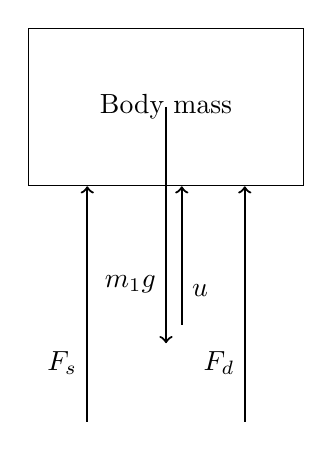
\begin{tikzpicture}
\node (M1) [draw, align=center, minimum width=3.5cm,minimum height=2cm] {Body mass};
\draw[->, thick] (M1.center) -- node[left, near end] {$m_1g$} ++(0, -3cm);
\draw[<-, thick] (M1.south) ++(-1cm, 0) -- node[left, near end] {$F_s$} ++ (0, -3cm);
\draw[<-, thick] (M1.south) ++(1cm, 0) -- node[left, near end] {$F_d$} ++ (0, -3cm);
\draw[<-, thick] (M1.south) ++(0.2cm, 0) -- node[right, near end] {$u$} ++ (0, -1.76cm);
\end{tikzpicture}
\end{center}
The equation of motion in the vertical direction becomes
\begin{equation}
 m_1 \ddot{z}_1 = \sum_i F_i = -m_1g + \underbrace{m_1g -k_1(z_1-z_2)}_{F_s} + \underbrace{\big(-b_1(\dot{z}_1 - \dot{z}_2) \big) }_{F_d} + u  = -k_1(z_1 - z_2) - b_1(\dot{z}_1 - \dot{z}_2) + u. 
 \label{eq:eom1}
 \end{equation}
On the suspension mass, there are five forces acting:
\begin{center}
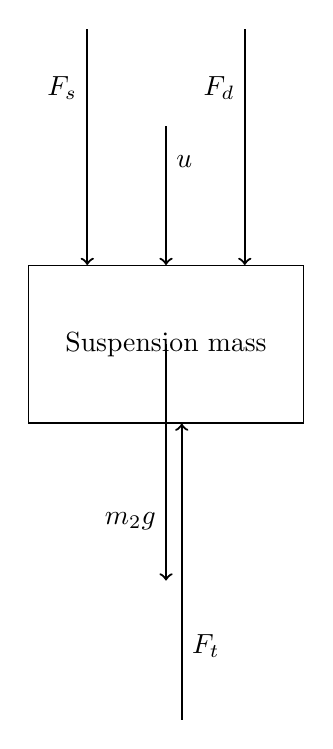
\begin{tikzpicture}
\node (M2) [draw, align=center, minimum width=3.5cm,minimum height=2cm] {Suspension mass};
\draw[->, thick] (M2.center) -- node[left, near end] {$m_2g$} ++(0, -3cm);
\draw[<-, thick] (M2.north) ++(-1cm, 0) -- node[left, near end] {$F_s$} ++ (0, 3cm);
\draw[<-, thick] (M2.north) ++(1cm, 0) -- node[left, near end] {$F_d$} ++ (0, 3cm);
\draw[<-, thick] (M2.north) ++(0cm, 0) -- node[right, near end] {$u$} ++ (0, 1.76cm);
\draw[<-, thick] (M2.south) ++(0.2cm, 0) -- node[right, near end] {$F_t$} ++ (0, -3.76cm);
\end{tikzpicture}
\end{center}
The equation of motion in the vertical direction becomes
\begin{equation}
\begin{split}
m_2\ddot{z}_2 &= -m2_g - \underbrace{\big(m_1g -k_1(z_1-z_2)\big)}_{F_s}
 - \underbrace{\big(- b_1(\dot{z}_1-\dot{z}_2)\big)}_{F_d}
 - \underbrace{\big( (m_1 + m_2)g - k_2(z_2 - w) \big)}_{F_t} - u\\
	       &= k_1(z_1 - z_2) + b_1(z_1 - z_2) - k_2(z_2-w) - u
 \end{split}
 \end{equation}

\item With the state vector 
\[ x = \bbm x_1\\x_2\\x_3\\x_4 \ebm = \bbm z_1 - z_2\\ \dot{z}_1 - \dot{z}_2 \\ z_2\\ \dot{z}_2 \ebm \]
we can write the four first-order differential equations of the state space model
 \begin{align*}
  \dot{x}_1 &= \dot{z}_1 - \dot{z}_2 = x_2\\
  \dot{x}_2 &= \ddot{z}_1 - \ddot{z}_2 = \frac{1}{m_1}\big( -k_1(z_1 - z_2) - b_1(\dot{z}_1 - \dot{z}_2) + u \Big) - \frac{1}{m_2} \Big(k_1(z_1 - z_2) + b_1(z_1 - z_2) - k_2(z_2-w) - u\Big)  \\
            &= -\Big(\frac{1}{m_1} + \frac{1}{m_2}\Big)k_1x_1 - \Big(\frac{1}{m_1} + \frac{1}{m_2}\Big)b_1x_2 + \frac{k_2}{m_2}x_3 - \frac{k_2}{m_2}w + \Big(\frac{1}{m_1} + \frac{1}{m_2}\Big) u\\
  \dot{x}_3 &= \dot{z}_2 = x_4\\
  \dot{x}_4 &= \ddot{z}_2 = \frac{1}{m_2} \Big( k_1(z_1 - z_2) + b_1(z_1 - z_2) - k_2(z_2-w) - u \Big)\\
            &= \frac{k_1}{m_2} x_1 + \frac{b_1}{m_2} x_2 - \frac{k_2}{m_2}x_3 + \frac{k_2}{m_2}w - \frac{1}{m_2}u.
\end{align*}
In state-space form, this can be written
\begin{align*}
\dot{x} &= \bbm 0 & 1 & 0 & 0\\ 
               -\Big(\frac{1}{m_1} + \frac{1}{m_2}\Big)k_1 & \Big(\frac{1}{m_1} + \frac{1}{m_2}\Big)b_1 & \frac{k_2}{m_2} & 0\\
               0 & 0 & 0 & 1\\
               \frac{k_1}{m_2} & \frac{b_1}{m_2} & - \frac{k_2}{m_2} & 0\ebm
               \bbm x_1\\x_2\\x_3\\x_4 \ebm + \bbm 0\\-\frac{k_2}{m_2}\\0\\\frac{k_2}{m_2} \ebm w + \bbm 0\\\frac{1}{m_1} + \frac{1}{m_2}\\0\\-\frac{1}{m_2} \ebm u \\
 y &= \bbm 1 & 0 & 0 & 0 \ebm x.
\end{align*}
\end{enumerate}






\subsection*{step-response}
\label{sec:orgheadline7}
The figure below shows the step-responses of both the continuous- and the sampled systems.
\begin{center}
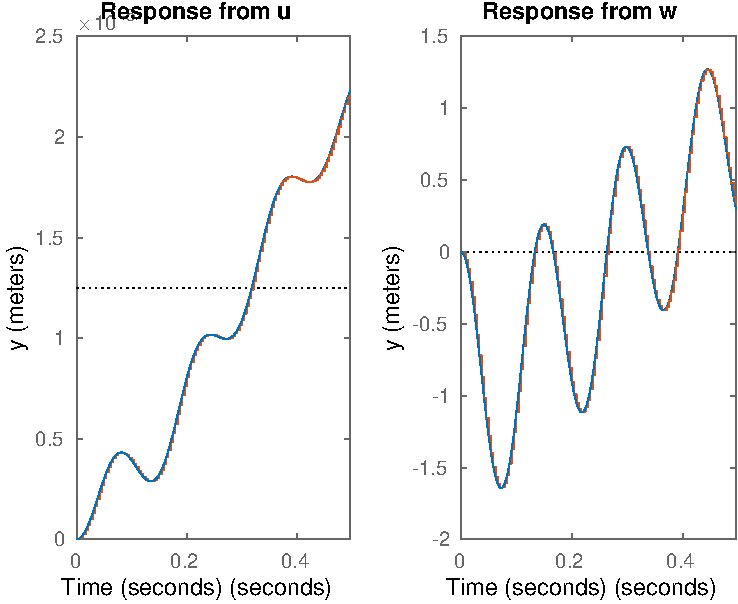
\includegraphics[width=0.6\linewidth]{active-susp-plant-response}
\end{center}

\subsection*{Sampling the system}
\label{sec:orgheadline8}
\begin{enumerate}
\item The fast oscillations in the beginning of the step-response have period \unit{0.13}{\second},  so the frequency is \(\omega_0 = \frac{2\pi}{0.13}\approx \unit{48}{\radians\per\second}\). This gives 
\[ h = \frac{0.2}{\omega_0} \approx \unit{0.0042}{\second}. \]
\item Sampling the system is straightforward 
\begin{verbatim}
sys_uy_d = c2d(sys_uy, h); % The system from input u to y
sys_wy_d = c2d(sys_wy, h); % From input w to y
\end{verbatim}
\end{enumerate}

\subsection*{Observability and reachability}
\label{sec:orgheadline9}
Obtain the \(\Phi\), \(\Gamma\), \(C\) and \(D\) matrices from the discretized system. Then form \(W_o\) and \(W_c\) and calculate the determinant
\begin{verbatim}
% Check observability and reachability
[Ad, Bd, Cd, Dd] = ssdata(sys_uy_d); 
Wo = [Cd;Cd*Ad;Cd*Ad*Ad; Cd*Ad*Ad*Ad]
det(Wo)
Wc = [Bd  Ad*Bd  Ad*Ad*Bd Ad*Ad*Ad*Bd]
det(Wc)
\end{verbatim}
The result is
\[ \det W_o = 1.26 \cdot 10^{-8}\]
and
\[ \det W_c = 5.92 \cdot 10^{-30}.\]

So, the system is observable, but not reachable. 
\end{document}